
\medskip

\begin{minipage}[b]{0.65\linewidth}
Sur la figure ci-contre :

\begin{itemize}[label=\textbullet]
\item les points E, A et F sont alignés;
\item les points E, B et D sont alignés;
\item les droites (FD) et (AB) sont parallèles;
\item $\mathrm{AE}=\np[cm]{4,4}$; $\mathrm{EB} =\np[cm]{3,3}$; $\mathrm{AB} = \np[cm]{5,5}$ et $\mathrm{BD} = \np[cm]{6,6}$.
\end{itemize}

\vspace{1cm}

\begin{enumerate}
\item Démontrer que le triangle ABE est rectangle.
\item Calculer la mesure de l'angle $\widehat{\mathrm{ABE}}$, arrondie au degré.
\item Calculer la longueur FD.
\end{enumerate}

\end{minipage}
\hfill
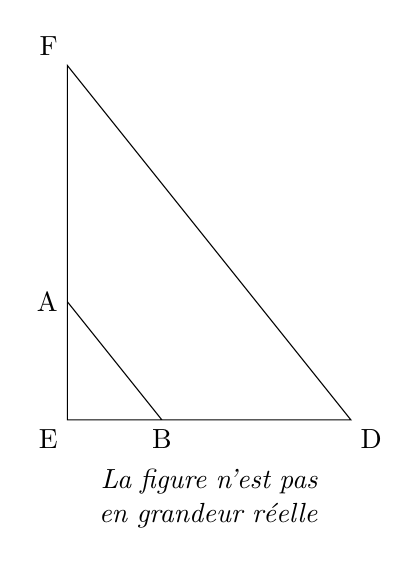
\begin{tikzpicture}[baseline={(current bounding box.south)}]
	\draw (0,0)node[below left]{E}--
		(3.6,0)node[below right]{D}--
		(0,4.5)node[above left]{F}-- cycle
		(0,1.5)node[left]{A}--
		(1.2,0)node[below]{B};
		\node[align=center,text width=3.6cm] at (1.8,-1)  {\emph{La figure n'est pas en grandeur réelle}};
\end{tikzpicture}

\begin{enumerate}[start=4]
\item Une homothétie de centre E transforme le triangle EAB en le triangle EFD.

Quel est le rapport de cette homothétie ? Aucune justification n'est attendue.
\end{enumerate}


